\documentclass[french,a4paper,10pt]{article}

\usepackage{graphicx}
\usepackage{xcolor}
\usepackage{comment}

\usepackage[utf8]{inputenc}
\usepackage[T1]{fontenc}
\usepackage{babel}

\usepackage{hyperref}
\hypersetup{
	colorlinks=true,
	linkcolor=black,
	urlcolor=blue,
}

\definecolor{codegreen}{rgb}{0,0.6,0}
\definecolor{codegray}{rgb}{0.5,0.5,0.5}
\definecolor{codepurple}{rgb}{0.58,0,0.82}
\definecolor{backcolour}{rgb}{0.95,0.95,0.92}

\usepackage{fancyhdr}
\usepackage{listings}

\lstdefinestyle{myPythonStyle}{
    backgroundcolor=\color{backcolour},
    commentstyle=\color{codegreen},
    keywordstyle=\color{magenta},
    numberstyle=\tiny\color{codegray},
    stringstyle=\color{codepurple},
    basicstyle=\ttfamily\footnotesize,
    breakatwhitespace=false,
    breaklines=true,
    captionpos=b,
    keepspaces=true,
    numbers=left,
    numbersep=5pt,
    showspaces=false,
    showstringspaces=false,
    showtabs=false,
    tabsize=4
}
\lstset{style=myPythonStyle}

\pagestyle{fancy}
\fancyhf{}
\rhead{Balistique des sports}
\lhead{STI2D}
\cfoot{Page \thepage}

\title{Petites notions de balistique des sports...}
\date{2020-06}
\author{A.D.G.}

% à utiliser pour compiler avec ou sans les réponses aux exercices, ie doc prof vs doc élève...
\includecomment{reponse}
%\excludecomment{reponse}

\begin{document}

\section*{Petites notions de balistique des sports...}

Un joueur d’un sport quelconque de ballon doit envoyer dans les cages adverses un tir depuis un endroit assez éloigné... Par exemple, la sonnerie de fin de match approche et le goal de handball de l’équipe adverse est sur le banc, les cages sont libres, le goal de l’autre équipe tente le coup depuis ses cages ! Sinon on part en prologation et il est fatigué...

Il sait qu’il peut envoyer le ballon à 72 km/h (surtout il sait que ça simplifie les calculs une fois dans la bonne unité), que le ballon pèse environ 450 g et que sa circonférence est de 60 cm. Le terrain mesure 40 m et les cages sont hautes de 2 m. 

La question qu’il se pose est : \og quel angle dois-je donner à mon tir pour que je sauve le match ? \fg{}. En fait c’est un scientifique dans l’âme et il se dit plutôt : \og quelle plage d’angles ai-je à ma disposition pour réaliser ce tir ? \fg{}. Alors commence dans sa tête tout une réfléxion et nous allons l’aider parce que sinon il va paniquer et tirer à coté !

\section{Hypothèses, vous avez dit hypothèses ?}
Nous allons commencer à nous intéresser à ce problème d'un point de vue scientifique afin de choisir les outils à utiliser et formuler les hypothèses qui vont nous permettre de résoudre.\\

\begin{enumerate}
    \item Quel est le système à isoler ?\\
\begin{reponse}
    \textcolor{red}{On isole le ballon (une fois qu’il a quitté les mains du goal...)}
\end{reponse}

    \item Quel outil va-t-on devoir utiliser pour résoudre ce problème ? Quelle est son équation ? \\
\begin{reponse}
\textcolor{red}{On utilise le principe fondamental de la dynamique (PFD), qui dit que la somme des forces appliquées à un solide isolé est égale à l’accélération multipliée par la masse du système. \\
PFD : $\Sigma \vec{F} = m . \vec{a}$}
\end{reponse}

    \item Quelles sont les forces qui s’appliquent sur le système ? Faisons un bilan des forces. \\
\begin{reponse}
\textcolor{red}{Le poids : $\vec{P} = m . \vec{g}$ dont la direction est la droite reliant le centre de gravité G du ballon et le centre de la Terre (évidemment dans notre cas on prend la verticale), et dont le sens est dirigé vers le centre de la Terre, donc vers le bas. \\
La poussée d'Archimède : $\vec{P_A} = \rho . Vol_{déplacé} . \vec{g}$\\
Les frottements de l’air : $\vec{T} = 1/2 . C_x . S_f . \rho . v^2 . \vec{u}$ qui est aussi un vecteur dont la direction est celle de la vitesse et dont le sens s'oppose au mouvement.}
\end{reponse}

    \item Quelles sont les forces que l’on néglige ? \\
\begin{reponse}
\textcolor{red}{Dans un premier temps, nous allons négliger les frottements de l’air car le ballon ne va pas très vite ainsi que la poussée d'Archimède car le ballon est beaucoup plus dense que l'air.}
\end{reponse}

    \item Écrire l’équation finale. \\
\begin{reponse}
\textcolor{red}{$P = m . a$ soit $-m . g = m . a$ (projeté sur l’axe vertical $\vec{z}$) donc $a(t) = -g$.}
\end{reponse}
\end{enumerate}

\section{Modélisation mathématique :}
Cette partie doit aboutir aux équations du mouvement du projectile, donc du ballon. Dans un premier temps on résoud ces équations en fonction du temps puis on termine par une description dans l'espace de la trajectoire.\\

\begin{enumerate}
    \item On se place dans un répère cartésien x, y, z... A-t-on vraiment besoin des trois dimensions ?\\
\begin{reponse}
\textcolor{red}{Non, il suffit de se placer dans le plan du tir, perpendiculaire au sol, donc on prendra un repère en deux dimensions z, x pour la suite.}
\end{reponse}

    \item Ecrire les équations de mouvement sur chacun des axes nécessaires et résoudre pour obtenir l’équation du mouvement en fonction du temps. (Indice : pensez à votre cours de sciences physiques !)\\
\begin{reponse}
\textcolor{red}{Si on utilise V\textsubscript{0} comme vitesse initiale et h\textsubscript{0} = 1.70 m (hauteur du bras du gardien) on obtient, après intégration et résolution des conditions initiales :\\
$x(t) = V_{0x} . t$\\
$z(t) = - 1/2 . g . t^2 + V_{0z} . t + h_0$\\
Démonstration :\\
Sur l'axe $\vec{x}$ :\\
$x"(t) = 0$\\
$x'(t) = k1$\\
$x(t) = k1 . t + k2$\\
Conditions initiales : pour $t = 0$ on a $x(0) = 0$ et $x'(0) = V_{0x}$. Donc $k1 = V_{0x}$ et $k2 = 0$.\\
Sur l'axe $\vec{z}$ :\\
$z"(t) = -g$\\
$z'(t) = -g . t + k1$\\
$z(t) = - 1/2 . g . t^2 + k1 . t + k2$\\
Conditions initiales : pour $t = 0$ on a $z(0) = h_0$ et $z'(0) = V_{0z}$. Donc $k1 = V_{0z}$ et $k2 = h_0$.}
\end{reponse}

    \item Combiner ces équations pour obtenir l’équation de la trajectoire dans le répère créé plus avant.\\
\begin{reponse}
    \textcolor{red}{$$z(x) = - 1/2 . g . \frac{x^2}{V_{0x}^2} + \frac{V_{0z}}{V_{0x}} . x + h_0$$}
\end{reponse}
\end{enumerate}

\section{Retour à notre problème d’angle...}
Le but premier de ce problème était de trouver quelle plage d'angles est à choisir pour tirer dans les cages adverses, il faut donc faire intervenir l'angle $\alpha$ dans nos équations...

\begin{enumerate}
    \item Peut-on résoudre directement l’équation pour trouver l’angle ? Quelles sont les données en x et z pour ce que l’on cherche ?\\
\begin{reponse}
    \textcolor{red}{V\textsubscript{0} est le vecteur vitesse initiale, de norme V\textsubscript{0} = 72 km/h, sens : vers les cages adverses (c'est mieux !), et direction : selon une droite qui fait un angle $\alpha$ avec l'horizontale.\\
$V_{0x} = V_0 . cos(\alpha)$\\
$V_{0z} = V_0 . sin(\alpha)$\\
Il faut remplacer dans l'équation précédente ce qui donne une équation du type :\\
$$z(x,\alpha) = - 1/2 . g . \frac{x^2}{(V_{0}. cos(\alpha))^2} + \frac{sin(\alpha)}{cos(\alpha)} . x + h_0$$\\
$$z(x,\alpha) = - 1/2 . g . \frac{x^2}{(V_{0}. cos(\alpha))^2} + tan(\alpha) . x + h_0$$\\
On ne peut pas la résoudre directement car on a des $cos^2$ et des $tan$ dans la même équation.\\
On peut en revanche se fixer à 40 m pour obtenir une équation $z = f(\alpha)$.}
\end{reponse}
    \item En utilisant un tableur (excel ou libreoffice calc) tracer la courbe de la trajectoire en se fixant des contraintes pour l’angle.\\
\begin{reponse}
\textcolor{red}{Ci-après on trouve les courbes de la trajectoire pour un angle $\alpha$ fixé à 20~° et de l'altitude du ballon à 40 m (au niveau des cages) pour des angles $\alpha$ variant de 30 à 55~°.}
\end{reponse}

    \item Utiliser une méthode similaire pour trouver une valeur approximative de la plage d’angle afin que notre joueur sauve le match et soit le héros du jour...\\
\begin{reponse}
\textcolor{red}{La plage de valeur est double, ce sont les valeurs de z comprises entre 0 et 2 m (hauteur des cages).\\
La première plage de valeur correspond à un tir \og tendu \fg{}, ensuite si on augmente l'angle on tire au dessus des cages puis on se met à tirer \og en cloche \fg{} et donc on retrouve une plage d'angles (mais plus faible car l'angle d'arrivée dans les buts est différent).}
\end{reponse}

    \item Ces valeurs vous paraissent-elles raisonnables ?\\
\begin{reponse}
\textcolor{red}{Outre le fait que l’on ne prend pas en compte le rebond du ballon c’est raisonnable.}
\end{reponse}

    \item Pour ce qui est du tir \og en cloche \fg{} quelle est la contrainte qui empêcherait le gardien de faire un tel tir et comment calculer les valeurs utiles pour répondre à cette question ?
\begin{reponse}
    \textcolor{red}{Si on joue sur un terrain en salle la hauteur du plafond limite le tir.\\
Il faut calculer donc hauteur maximale du ballon à l'apogée de la trajectoire. Pour cela on utilise la dérivée de la trajectoire et on cherche la valeur pour laquelle celle-ci s'annule. Mathématiquement cela signifie que la tangeante à la courbe est horizontale.\\
On peut aussi reprendre l'équation $z = f(t)$ et effectuer le même calcul. Physiquement ou mécaniquement cela correspondrait au moment où la vitesse projetée sur l'axe $\vec{z}$ s'annule. Le ballon monte de plus en plus lentement puis \og s'arrête \fg{} et redescend.
Formule et application numérique :\\
$$z(x,\alpha) = - 1/2 . g . \frac{x^2}{(V_{0}. cos(\alpha))^2} + tan(\alpha) . x + h_0$$\\
$$z'(x,\alpha) = - g . \frac{x}{(V_{0}. cos(\alpha))^2} + tan(\alpha)$$\\
d'où si $z'(x) = 0$ on a $x = (V_0 . cos(\alpha))^2 . tan(\alpha) / g$\\
si $V_0 = 72$ km/h et $\alpha = 53$~°, x = 19.59 m et z = 14.70 m... Pour un gymnase standard ça doit être trop haut sans doute...}
\end{reponse}

    \item Comment pensez-vous que ces valeurs évolueraient sans les hypothèses que nous avons faites au début ?\\
\begin{reponse}
\textcolor{red}{On aurait sans doute des valeurs différentes en prenant en compte les frottements mais celles-ci ne sont pas déraisonnables.}
\end{reponse}

\end{enumerate}

\section{Optimisation, le nerf de la guerre...}
Maintenant que nous avons bien saisi tout le problème et ses variables, il serait intéressant de savoir quel est l'angle le plus approprié pour utiliser le moins de force possible pour ce tir. Cela correspond, mathématiquement à chercher le minimum de la variable V\textsubscript{0} en fonction de l'angle $\alpha$.

\begin{enumerate}
    \item Quelle est l'équation à utiliser pour trouver ces informations ?\\
\begin{reponse}
\textcolor{red}{$$z(x,\alpha,V_0) = - 1/2 . g . \frac{x^2}{(V_{0}. cos(\alpha))^2} + tan(\alpha) . x + h_0$$\\
Attention, ici nous avons $z = f(x,\alpha,V_0)$, les trois valeurs sont des variables...}
\end{reponse}

    \item Quelles sont les valeurs de z et de x à fixer ?\\
\begin{reponse}
\textcolor{red}{Pour x c'est très simple, x = 40 m donc au niveau des cages adverses...\\
Pour z il y a une plage de valeur, z = [0 ; 2]. Ici on cherche la vitesse V\textsubscript{0} la plus faible donc \emph{a priori} z = 0 nécessitera une vitesse moindre (c'est une hypothèse qu'il conviendrait de vérifier).}
\end{reponse}

    \item En utilisant à nouveau un tableur, trouver une approximation de la vitesse optimale, donc minimale (cela demandera le moins de puissance bien-sûr), pour le tir. Quelle est la formule à utiliser ? \\
\begin{reponse}
    \textcolor{red}{On a :\\
$$z(x,\alpha,V_0) = - 1/2 . g . \frac{x^2}{(V_{0}. cos(\alpha))^2} + tan(\alpha) . x + h_0$$ avec x = 40 et z = 0.\\
 Cela peut s'écrire $ z(40,\alpha,V_0) = 0$ et on obtient la formule $V_0 = f(\alpha)$ :\\
$$V_0 = \sqrt{\frac{1/2 . g . 40^2}{cos^2(\alpha) . (h_0 + 40 . tan(\alpha))}}$$\\
Il faut ensuite regarder sur la courbe $V_0 = f(\alpha)$ où se situe la valeur minimale pour V\textsubscript{0}. A l'oeil on trouve environ 70 km/h pour 44~°. En faisant le même travail pour z = 2 m on trouve des valeurs très similaires...}
\end{reponse}

\end{enumerate}

\section{La réponseur du codeur au mécanicien !}
Les formules trouvées sont trop compliquées pour faire une résolution numérique mais on peut trouver des solutions approchées, c'est d'ailleurs ce que l'on fait lorsque l'on regarde dans le tableurs et sur les courbes.

Il existe plusieurs méthodes mathématiques et algorythmiques pour trouver des valeurs approchées d'équations, nous allons voir la plus simple d'entre elles : la méthode par \og dychotomie \fg{}. Cette méthode très robuste mais pas très efficace/rapide nécessite quelques hypothèses. Si l'on cherche la résultat $x$ pour $f(x) = 0$, la fonction f traitée doit être continue et monotone sur l'intervalle de recherche [a ; b], et $f(a)$ et $f(b)$ doivent être de signe opposés. Si on cherche $f(x) = k$ il est évidemment similaire de chercher $g(x) = f(x) -k = 0$.

La méthode par dychotomie consiste à réduire l'intervalle de recherche de solution par deux à chaque itération en changeant soit le début soit la fin de l'intervalle par son milieu.\\
Sur [a ; b], le milieu m correspond à $m = (a+b)/2$.\\
On cherche $f(a)$, $f(b)$ et $f(m)$ et on regarde lequel de $f(a)$ ou $f(b)$ est de signe opposé à $f(m)$ ce qui nous donne l'intervalle suivant [a, m] ou [m, b]. Et on recommence...

Cette méthode est une méthode numérique donc on obtient une solution approximative et donc il faut se fixer une précision, une valeur pour laquelle on arrête les itérations. Ici c'est l'écart entre les valeurs de l'intervalle de recherche de solution qui donne la précision, l'écart vaut $\epsilon = b - a$ et donc si $\epsilon$ est inférieur à la précision cela signifie que la prochaine itération n'améliorera pas le résultat final et on peut arrêter.

\begin{enumerate}
    \item En repensant à la partie où l'on cherche l'apogée de la trajectoire et la hauteur au plus haut, trouver une méthode permettant de chercher l'angle pour lequel on obtient une vitesse optimale donc minimale.\\
\begin{reponse}
\textcolor{red}{On cherche l'endroit où la courbe $V_0 = f(\alpha)$ est à son point mini. Pour cette courbe c'est le point où la tangeante est horizontale (comme pour la trajectoire) et donc le point où la dérivée $f'(\alpha)$ s'annule.\\
Il faut donc calculer la dérivée de V\textsubscript{0} en fonction de $\alpha$. Ce qui n'est pas une mince affaire !\\
L'équation de $dV_0 / d\alpha$ est la suivante :
$$\frac{dV_0}{d\alpha} = \frac{-40.\sqrt{1/2.g}.(-2.sin(\alpha).(h_0 + 40.tan(\alpha)) + 40.cos(\alpha).(1+tan^2(\alpha)))}{2.cos^2(\alpha).(h_0+40.tan(\alpha))^{3/2}}$$}
\end{reponse}

    \item Proposer un algorithme (ou un algorigramme) de la méthode de recherche de solution par dychotomie.\\
\begin{reponse}
\textcolor{red}{TBDone}
\end{reponse}

    \item Coder en python la méthode et tester votre programme pour une fonction \og facile \fg{} et dont on connait le résultat, par exemple $f(x) = 0.3 * x^2 - 7$.\\
\begin{reponse}
\textcolor{red}{Exemple de code pour ce programme :}
\begin{lstlisting}[language=python]
def fonction(x):
    y = 0.3 * x**2 - 7 
    return y

def dychotomie(f, a, b, k, epsilon):
     # cas d'une fonction croissante monotone sur l'intervalle
     debut = a
     fin = b
     ecart = b - a
     iteration = 0
     while ecart > epsilon:
         milieu = (debut + fin) / 2
         if f(milieu) > k:
             # la solution est < m
             fin = milieu
         else:
             # la solution est > m
             debut = milieu
         ecart = fin - debut
         iteration += 1
     return milieu, iteration

result, iteration = dychotomie(fonction, 0, 10, 0, 0.001)
print('resultat :',result, '(en', iteration, 'iterations, avec une precision au millieme)')
\end{lstlisting}
\textcolor{red}{Le programme rend le résultat suivant :\\
résultat : 4.8309326171875 (en 14 itérations, avec une précision au millième)}
\end{reponse}

    \item Chercher la solution à la question principale de cette activité : quelle est l'angle qui permet d'avoir à donner la vitesse minimale au ballon et qu'elle est cette vitesse ?\\
\begin{reponse}
    \textcolor{red}{Voir le fichier html produit par \emph{Jupyter Notebook} pour les codes et calculs... La valeur approximative à 0.001 est $\alpha = 43.777$ \textdegree.} 
\end{reponse}

\end{enumerate}

\begin{reponse}
\textcolor{red}{\section{Annexe : courbes réponses faites avec LibreOffice Calc}}
\begin{figure}[h]
    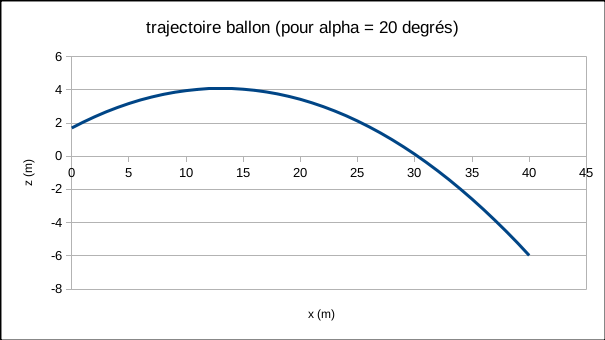
\includegraphics[width=.8\linewidth]{courbe_trajectoire.png}
    \caption{Trajectoire du ballon pour une vitesse initiale de 72 km/h et un angle de tir de 20~°}
\end{figure}

\begin{figure}[h]
    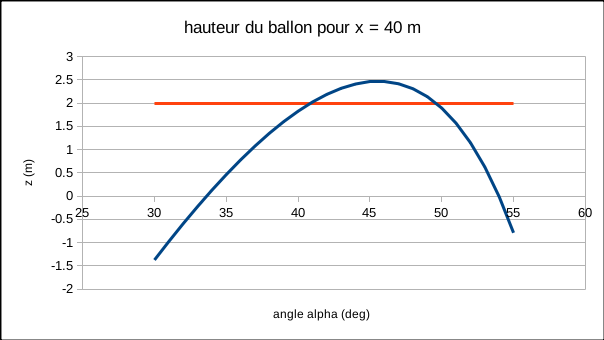
\includegraphics[width=.8\linewidth]{courbe_alpha.png}
    \caption{Visualisation de la hauteur du ballon en fonction de l'angle de tir par rapport à la barre transversale (en rouge) à 40 m, donc au niveau des cages à l'autre bout du terrain. La vitesse initiales est toujours de 72 km/h.}
\end{figure}

\begin{figure}[h]
    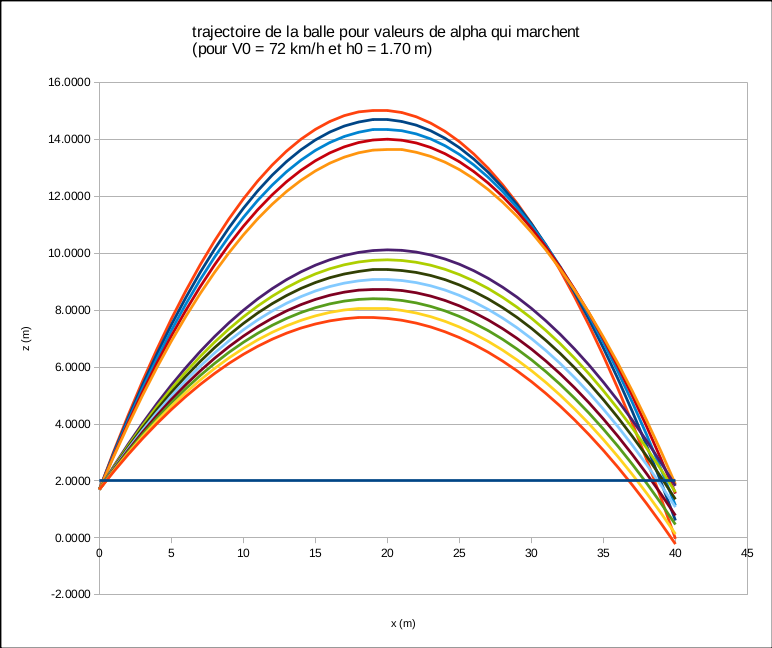
\includegraphics[width=.8\linewidth]{courbe_trajectoires_alpha.png}
    \caption{Faisceau de trajectoire du ballon pour un tir à 72 km/h. Seules sont représentées les courbes pour le cas où le ballon entre dans les cages (sans rebond), pour $\alpha$ = [33 ; 40] \& $\alpha$ = [50 ; 54].}
\end{figure}

\begin{figure}[h]
    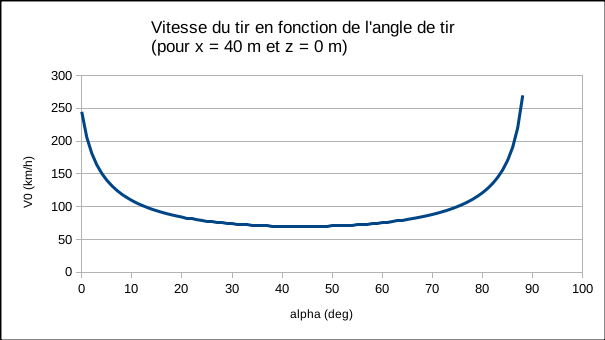
\includegraphics[width=.8\linewidth]{courbe_V0@0.png}
    \caption{Optimisation de la vitesse de tir en fonction de l'angle de tir pour une hauteur d'entrée dans les cages de 0 m, soit le ballon arrive au sol sur la ligne...}
\end{figure}

\begin{figure}[h]
    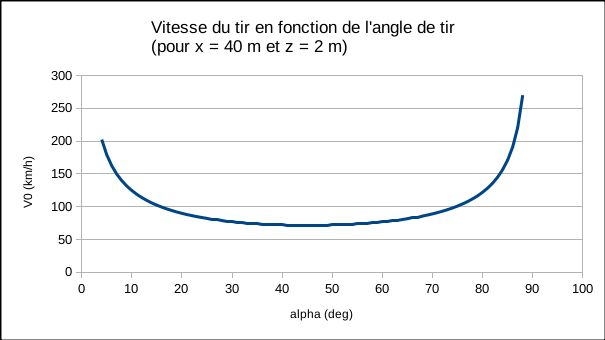
\includegraphics[width=.8\linewidth]{courbe_V0@2.png}
    \caption{Optimisation de la vitesse de tir en fonction de l'angle de tir pour une hauteur d'entrée dans les cages de 2 m, soit le ballon arrive juste sous la barre transversale.}
\end{figure}
\end{reponse}

\end{document}
